\documentclass[crop,tikz]{standalone}
\usetikzlibrary{shapes}
\usetikzlibrary{arrows}
\usetikzlibrary{positioning}

\begin{document}
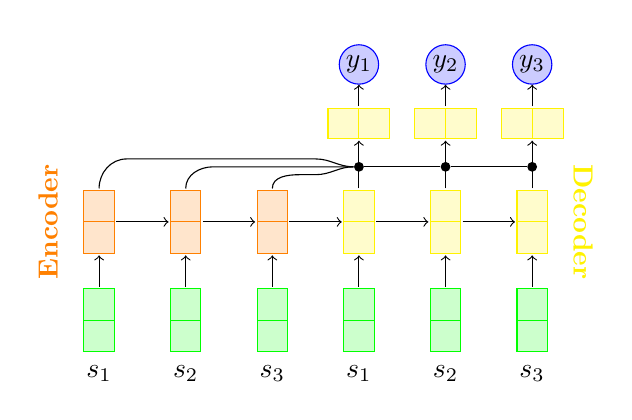
\begin{tikzpicture}[
  hid/.style 2 args={
    rectangle split,
    draw=#2,
    rectangle split parts=#1,
    fill=#2!20,
    outer sep=.25mm},
  mlp/.style 2 args={
    rectangle split,
    rectangle split horizontal,
    draw=#2,
    rectangle split parts=#1,
    fill=#2!20,
    outer sep=.25mm}
]

 % Comment out this line to remove border.
 \draw[draw=white] (-3.1, 4.21) rectangle (4.2, -.4);

 \foreach \step in {1,...,3} {
   \node (ie\step) at (1.1*\step - 3.3, -.18) {$s_\step$};
   \node[hid={2}{green}] (se\step) at (1.1*\step - 3.3, .5) {};    
   \node[hid={2}{orange}] (he\step) at (1.1 *\step - 3.3, 1.75) {};    
   \draw[->] (se\step.north) -> (he\step.south);
 } 

 \node[rotate=90,orange] at (-2.85, 1.75) {\textbf{Encoder}};
 \node[rotate=-90,yellow] at (3.95, 1.75) {\textbf{Decoder}};

 \foreach \step in {1,...,3} {
   \node (id\step) at (1.1*\step, -.18) {$s_\step$};
   \node[hid={2}{green}] (sd\step) at (1.1*\step, .5) {};    
  
   \node[hid={2}{yellow}] (hd\step) at (1.1 *\step, 1.75) {};    
   \draw[->] (sd\step.north) -> (hd\step.south);

   \node[mlp={2}{yellow}] (g\step) at (1.1 *\step, 3.0) {};    
   \node[circle, draw=blue, fill=blue!20,minimum size=5mm] (y\step) 
       at (1.1 *\step, 3.75) {};
   \node at (1.1 *\step, 3.75) {$y_\step$};    
   \draw[->] (g\step.north) -> (y\step.south);
   \draw[->] (hd\step.north) -> (g\step.south);
   \node[circle,fill,inner sep=1.25pt] (t\step) at (1.1 * \step, 2.45) {};
 }


 \draw[-] (he1.north) to [out=90,in=180] (-1.85, 2.55) to (0.55, 2.55) 
    to [out=0,in=180] (t1.west); 
 \draw[-] (he2.north) to [out=90,in=180] (-0.75, 2.45) to (0.55, 2.45) 
    to [out=0,in=180] (t1.west); 
 \draw[-] (he3.north) to [out=90,in=180] (0.35, 2.35) to (0.55, 2.35) 
    to [out=0,in=180] (t1.west); 
 \draw[-] (t1.east) to (t2.west);
 \draw[-] (t2.east) to (t3.west);

 \foreach \last/\next in {1/2, 2/3} {
   \draw[->] (he\last.east) -> (he\next.west);
   \draw[->] (hd\last.east) -> (hd\next.west);
 }
 \draw[->] (he3.east) -> (hd1.west);


\end{tikzpicture}
\end{document}
